\chapter{METODOLOGÍA: DESIGN THINKING}
El presente capítulo describe la metodología que guía el desarrollo del proyecto. El desarrollo de una aplicación móvil orientada al bienestar emocional no puede limitarse a decisiones técnicas o estéticas; requiere una metodología que coloque al usuario en el centro del proceso desde su inicio. En este sentido, la combinación del Design Thinking con el diseño de Experiencia de Usuario (UX) constituye el enfoque metodológico que sustenta el presente proyecto, ya que ambos comparten una orientación común: comprender profundamente al usuario para diseñar soluciones que respondan a sus necesidades reales y no a suposiciones del equipo de desarrollo (Vargas Márquez et al., 2021). Para ello, se abordan en primer lugar la definición y el origen del Design Thinking; en segundo lugar, sus características y los principales modelos que lo describen; en tercer lugar, las cinco etapas del modelo adoptado; en cuarto lugar, su relación con el diseño de experiencia de usuario; y, finalmente, la forma en que se aplicó en el presente proyecto.

\section{DEFINICIÓN Y ORIGEN DEL DESIGN THINKING}
El Design Thinking, o pensamiento de diseño, es definido por Vargas Márquez et al. (2021) como ``un modelo de cómo enfocar la innovación en entornos inciertos de forma ágil y radical'' (p. 11), compuesto por una serie de herramientas que se utilizan a lo largo del proceso de crear productos y servicios innovadores, en función de la fase en la que se encuentre el equipo. Los autores añaden que ``se puede utilizar Design Thinking siempre, porque tiene su base en la resolución de problemas, desde el punto de vista del usuario'' (p. 11).

Brown y Wyatt (2010), de la consultora de diseño IDEO, lo describen como un nuevo enfoque para crear soluciones que ``incorpora en profundidad la comprensión de los usuarios o consumidores y la creación rápida de prototipos, todo ello orientado a superar los supuestos que bloquean las soluciones eficaces'' (p. 29; traducción propia). Según estos autores, el enfoque se originó en la práctica profesional del diseño: IDEO se formó en 1991 a partir de la fusión de David Kelley Design y de ID Two, y en sus inicios se dedicó al diseño tradicional de productos; sin embargo, hacia 2001 comenzó a recibir encargos alejados del diseño tradicional, como reestructurar una organización o crear entornos de aprendizaje alternativos al aula, lo que la llevó a pasar del diseño de productos de consumo al diseño de experiencias (Brown \& Wyatt, 2010, pp. 29--30).

Un rasgo central del Design Thinking es su naturaleza humana. Brown y Wyatt (2010) señalan que el enfoque ``no solo se centra en crear productos y servicios centrados en las personas, sino que el proceso en sí mismo también es profundamente humano'' (p. 30; traducción propia), ya que se apoya en la capacidad de las personas para ser intuitivas, reconocer patrones y ``construir ideas que tengan significado emocional además de ser funcionales'' (p. 30; traducción propia). Este último aspecto resulta especialmente pertinente para el presente proyecto, cuyo propósito no es solo que la aplicación funcione, sino que genere experiencias emocionalmente significativas entre los jóvenes.

\section{CARACTERÍSTICAS DEL DESIGN THINKING}
A partir de las fuentes revisadas, pueden identificarse las siguientes características del Design Thinking:

\begin{itemize}
    \item \textbf{Centrado en las personas.} Vargas Márquez et al. (2021) señalan que ``generar empatía con nuestros clientes implica poner sus problemas, más que nuestras soluciones, en primer lugar'' (p. 7), y que el Design Thinking ``se centra en las personas, considerando multidisciplinariedad, colaboración y concreción de pensamientos y procesos, los cuales son caminos que llevan a soluciones innovadoras'' (p. 8).
    \item \textbf{Iterativo y no lineal.} Brown y Wyatt (2010) sostienen que el proceso ``se entiende mejor como un sistema de espacios superpuestos, más que como una secuencia de pasos ordenados'' (p. 30; traducción propia), ya que un proyecto puede volver más de una vez sobre sus distintos espacios a medida que el equipo refina sus ideas y explora nuevas direcciones (p. 30). Del mismo modo, Vargas Márquez et al. (2021) advierten que la evaluación puede revelar que el error no estaba solo en la solución, sino también en la forma de enmarcar el problema (p. 14).
    \item \textbf{Divergente y convergente.} El proceso alterna momentos en los que se amplían las opciones y momentos en los que se seleccionan. Vargas Márquez et al. (2021) indican que en la etapa de idear ``es necesario también separar el área de generación de ideas con el área de evaluación de ideas'' (p. 13), y Brown y Wyatt (2010) recomiendan postergar el juicio durante la lluvia de ideas, generar tantas ideas como sea posible y, después, agruparlas y ordenarlas (p. 31).
    \item \textbf{Aprendizaje a través del prototipado y del error temprano.} Brown y Wyatt (2010) identifican el miedo al fracaso como uno de los mayores impedimentos para adoptar el enfoque, y plantean que la experimentación y el error no son un problema siempre que ocurran temprano y sirvan como fuente de aprendizaje; por ello, una cultura de Design Thinking promueve ``el prototipado (rápido, barato y tosco) como parte del proceso creativo y no solo como una forma de validar ideas terminadas'' (p. 43; traducción propia).
\end{itemize}

\section{MODELOS DEL DESIGN THINKING}
El Design Thinking no cuenta con un único modelo de proceso. Vargas Márquez et al. (2021) analizan tres modelos reportados en la literatura, a fin de resaltar sus similitudes y su relación con la resolución creativa de problemas (p. 15):

\begin{itemize}
    \item \textbf{Modelo Divergente-Convergente (DCIDT).} Describe el pensamiento de diseño como divergente o convergente: los requisitos de diseño se transforman, mediante preguntas de diseño generativo, en una serie de conceptos de diseño, que posteriormente se convierten en decisiones o especificaciones de diseño mediante preguntas de razonamiento profundo, cuyo propósito es analizar, evaluar y validar dichos conceptos (Vargas Márquez et al., 2021, p. 15).
    \item \textbf{Modelo de Dunne y Martin.} Consta de cuatro actividades: abducción, deducción, prueba e inducción. En la abducción se generan ideas; en la deducción, esas ideas se analizan para predecir sus posibles consecuencias; las predicciones se ponen a prueba; y el resultado válido se generaliza en la etapa de inducción (Vargas Márquez et al., 2021, pp. 15--16).
    \item \textbf{Modelo de Brown.} Describe el pensamiento de diseño por medio de tres espacios superpuestos: inspiración, ideación e implementación (Vargas Márquez et al., 2021, p. 16). Brown y Wyatt (2010) definen la inspiración como el problema u oportunidad que motiva la búsqueda de soluciones; la ideación, como el proceso de generar, desarrollar y probar ideas; y la implementación, como el camino que lleva la solución desde la etapa de proyecto hasta la vida de las personas (p. 30).
\end{itemize}

Según Vargas Márquez et al. (2021), estos tres modelos comparten características comunes, ``como la exploración contextual holística, la generación de ideas basadas en el pensamiento integrador, la creación y evaluación de soluciones viables y la realización de soluciones en el contexto'' (p. 16). El presente proyecto adopta el modelo de cinco etapas (empatizar, definir, idear, prototipar y testear) que Vargas Márquez et al. (2021) describen a partir de la guía de Plattner (2018, como se citó en Vargas Márquez et al., 2021), dado que su estructura por etapas, con técnicas específicas para cada una, permite documentar con claridad cómo cada decisión de diseño se deriva de la evidencia recogida con los usuarios.

\section{ETAPAS DEL DESIGN THINKING}
El modelo adoptado consta de cinco etapas principales: empatizar, definir, idear, prototipar y testear; las cuales no son lineales sino iterativas, ya que la evaluación puede revelar la necesidad de volver a fases anteriores, incluso para reformular el problema (Vargas Márquez et al., 2021, p. 14). La Figura \ref{fig:design_thinking} representa estas etapas.

\begin{figure}[htbp]
  \centering
  \caption{Etapas del Design Thinking}
  \label{fig:design_thinking}
  \vspace{4pt}
  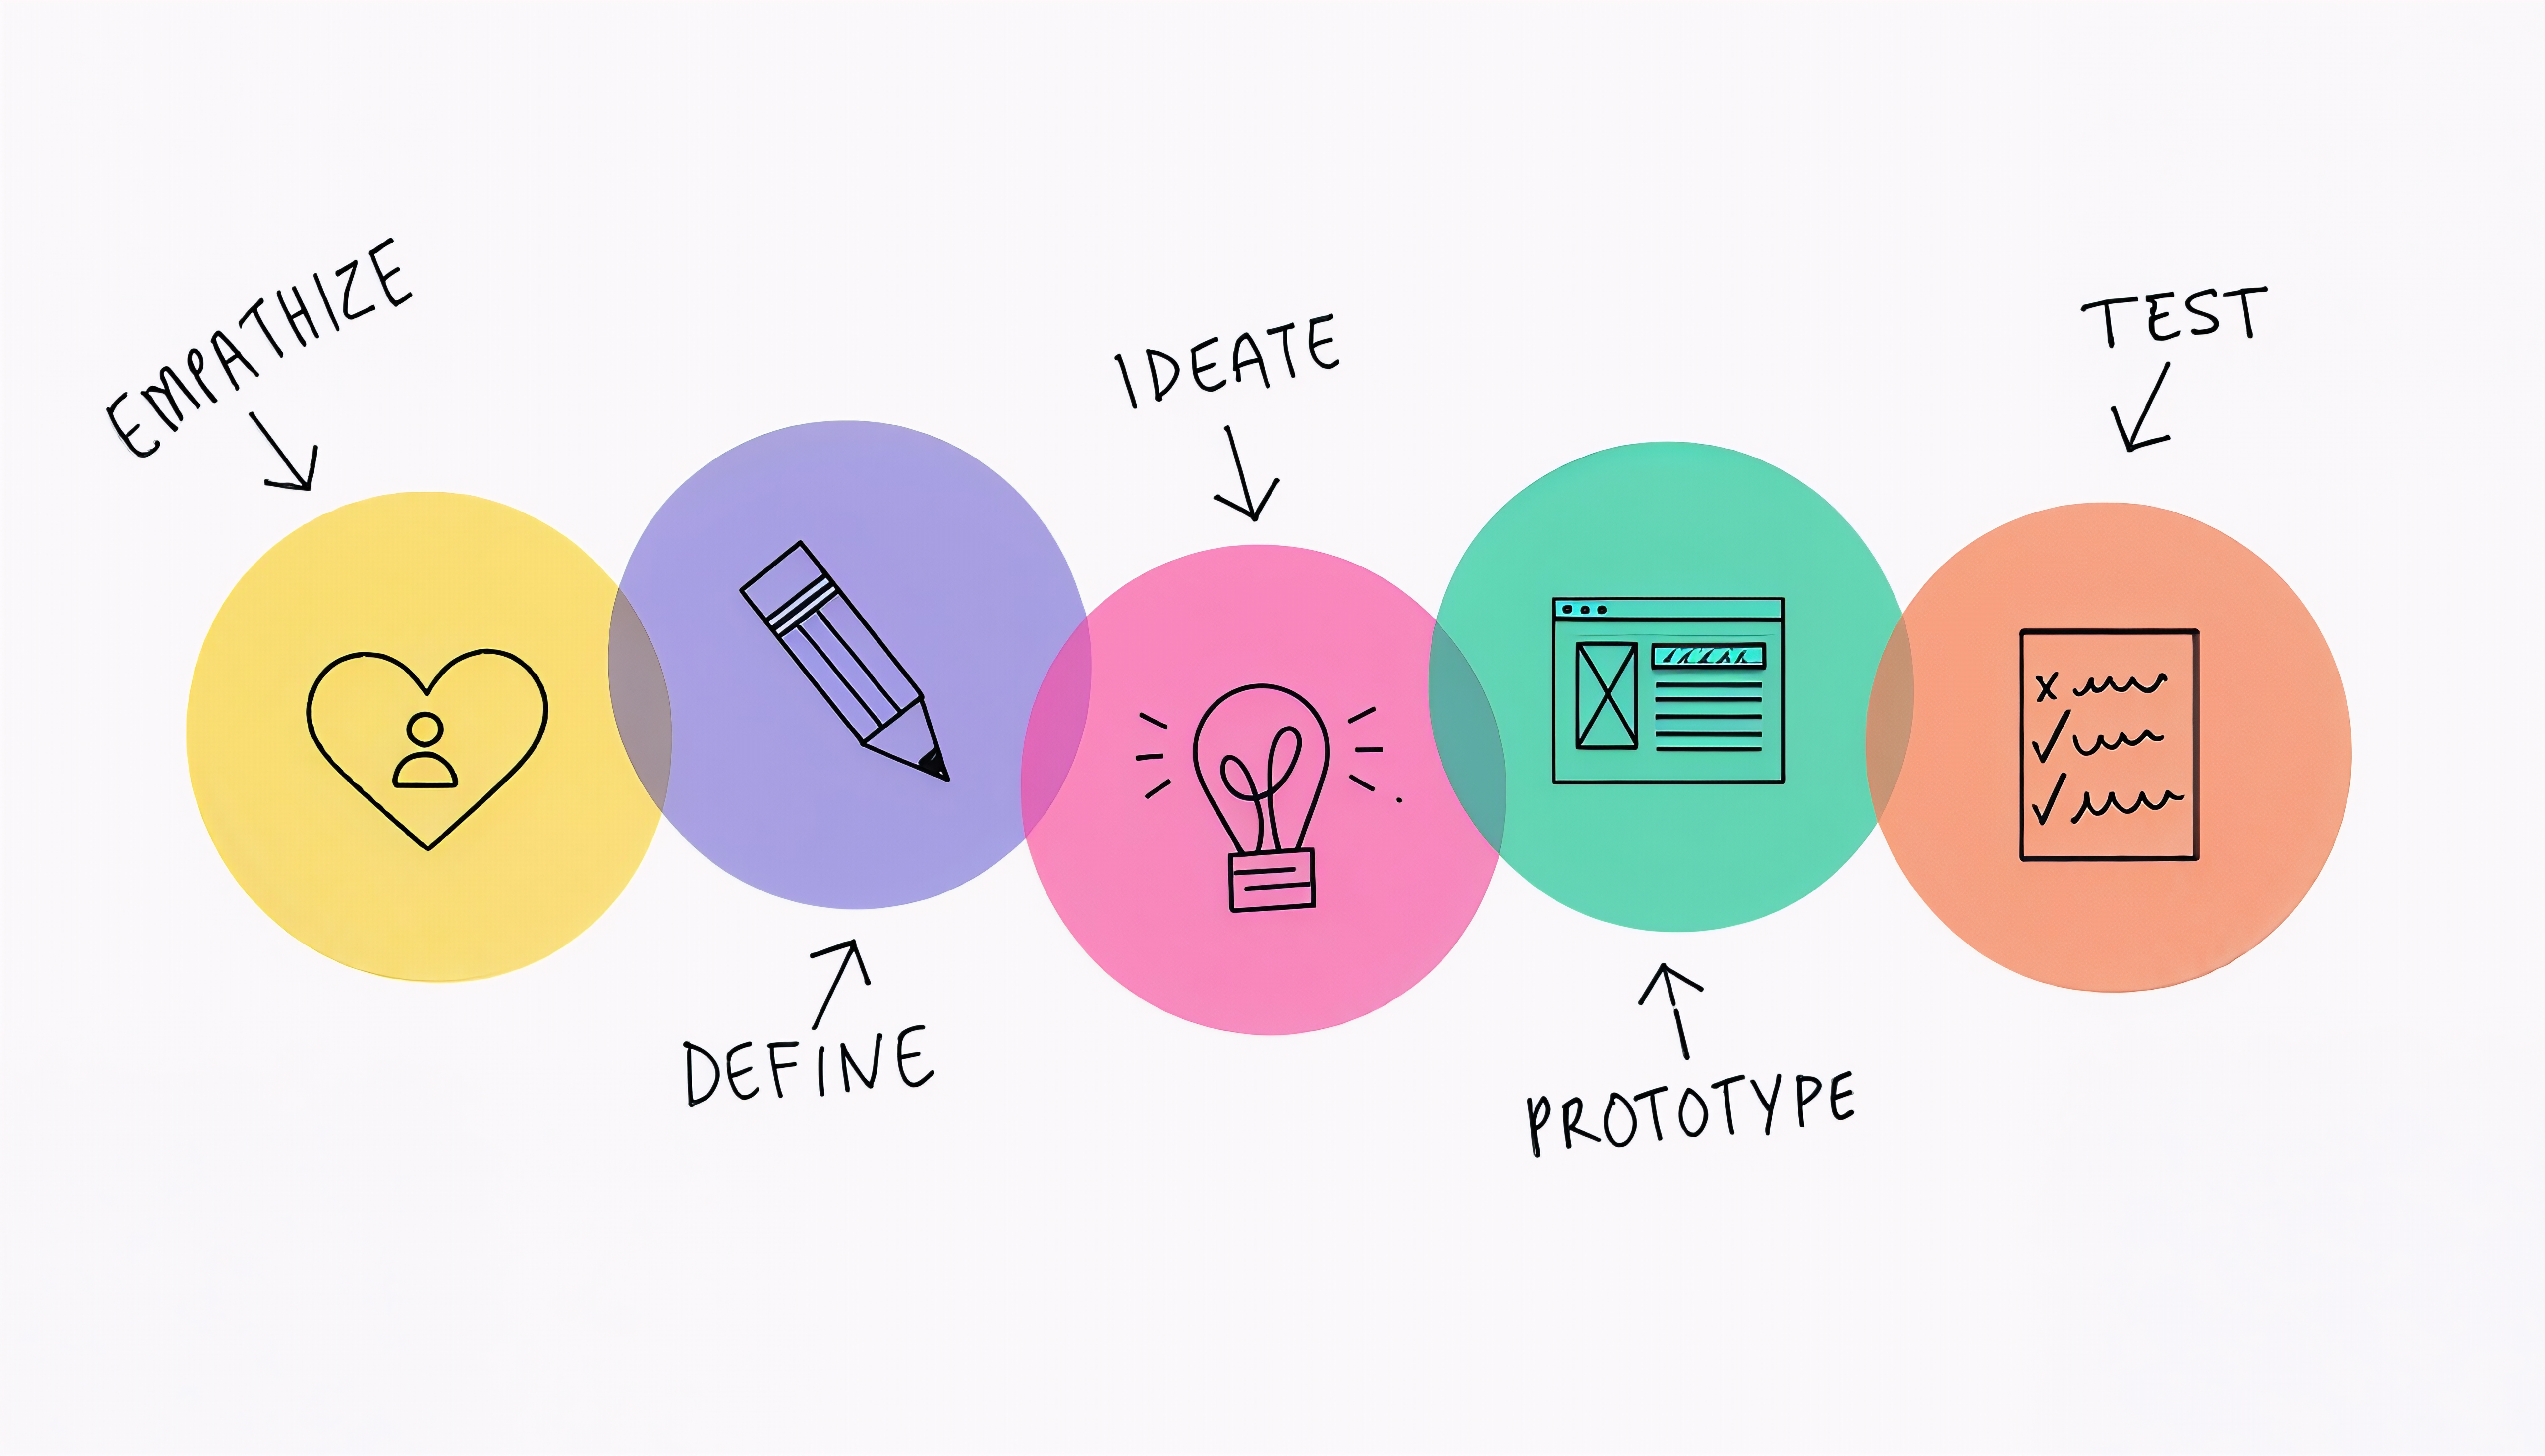
\includegraphics[width=0.7\textwidth]{Images/document/designThinking.jpg}
  \vspace{4pt}
\end{figure}

\begin{itemize}
    \item La primera etapa, empatizar, constituye la base de todo el proceso. Implica observar a los usuarios en su contexto, involucrarse en conversaciones con ellos y escuchar activamente sus necesidades, motivaciones y frustraciones. Vargas Márquez et al. (2021) señalan que ``los problemas que tratas de resolver no son los tuyos, son problemas de otras personas. Para diseñar para estas personas debes adquirir la empatía por lo que ellos son como personas y lo que es importante para ellos'' (p. 12). Al conversar con los usuarios, los autores recomiendan que ``lo importante es siempre preguntar `¿Por qué?' ya que eso descubre nuevos significados'' (pp. 11--12). Los autores denominan a esta etapa \textit{immerse}, ``ya que el diseñador debe hundirse en un mar de aprendizaje'' (p. 12).
    \item La segunda etapa, definir, consiste en sintetizar la información recopilada durante la fase anterior para construir un planteamiento del problema claro y orientado al usuario. Vargas Márquez et al. (2021) la describen como el momento de ``crear coherencia sobre la variada información que se ha reunido'' (p. 12), con el objetivo de formular un Point of View (POV) que guíe las decisiones de diseño subsiguientes. Este POV debe enmarcar el problema con un enfoque directo, ser inspirador para el equipo y capturar las mentes y corazones de las personas estudiadas (p. 12).
    \item La tercera etapa, idear, abre el espacio a la generación de múltiples soluciones posibles. En ella se desarrollan lluvias de ideas (\textit{brainstorms}) y se puede trabajar con métodos como croquis, mapas mentales, prototipos y \textit{storyboards} (Vargas Márquez et al., 2021, p. 13). Según los autores, la creación de múltiples ideas permite, entre otros aspectos, ``aprovechar de mejor manera las distintas visiones de cada equipo de trabajo y el trabajo colectivo'' (p. 13), así como aumentar el potencial de innovación del conjunto de posibilidades.
    \item La cuarta etapa, prototipar, implica la construcción de representaciones tangibles de las soluciones propuestas. Vargas Márquez et al. (2021) destacan que ``si una imagen vale mil palabras, un prototipo vale mil imágenes'' (p. 13), ya que permite comunicar, iniciar conversaciones con los usuarios y cometer errores de manera temprana y económica. Los prototipos deben ser rápidos y baratos de hacer, y se van refinando a medida que el proyecto avanza (p. 13).
    \item La quinta etapa, testear, consiste en solicitar retroalimentación sobre los prototipos a los propios usuarios. Vargas Márquez et al. (2021) recomiendan ``siempre hacer un prototipo creyendo que estamos en lo correcto, pero debemos evaluar pensando que estamos equivocados'' (p. 14), lo que garantiza una actitud crítica y abierta a la mejora continua. Entre sus recomendaciones para evaluar se encuentra entregar el prototipo a los usuarios ``sin explicar nada'' y observar cómo lo interpretan y lo usan (p. 14). Esta etapa no solo sirve para refinar el prototipo, sino también para aprender más sobre el usuario y, en ocasiones, para reformular el planteamiento del problema (p. 14).
\end{itemize}

\section{DESIGN THINKING Y DISEÑO DE EXPERIENCIA DE USUARIO}
El diseño de experiencia de usuario (UX \textit{Design}) comparte con el Design Thinking su carácter iterativo. Según Montero (2015, como se citó en Vargas Márquez et al., 2021), la principal diferencia del UX \textit{Design} frente a otros enfoques ``es que su proceso no es secuencial o lineal, sino que presenta ciclos en los que iterativamente se prueba el diseño y se optimiza hasta alcanzar el nivel de calidad requerido'' (p. 10). Este proceso comprende las fases de planificación o investigación, diseño o prototipado, evaluación, implementación y monitorización (Montero, 2015, como se citó en Vargas Márquez et al., 2021, pp. 10--11).

Vargas Márquez et al. (2021) plantean que el problema que se busca resolver en el diseño de experiencia de usuario ``es que el diseñador no sabe si el usuario encontrará amigable la interfaz propuesta para este, es por eso que Design Thinking es una de los métodos más usados con el fin de ponerse en la posición del usuario final'' (p. 17). A partir de ello, los autores proponen vincular cada fase del diseño de experiencia de usuario con una etapa del Design Thinking, tal como se resume en la Tabla \ref{tab:dt_ux}.

\begin{table}[htbp]
\caption{Correspondencia entre las fases del diseño de experiencia de usuario y las etapas del Design Thinking}
\label{tab:dt_ux}
\begin{tabular}{
  >{\raggedright\arraybackslash}p{0.22\textwidth}
  >{\raggedright\arraybackslash}p{0.22\textwidth}
  >{\raggedright\arraybackslash}p{0.46\textwidth}
}
\toprule
\textbf{Fase de UX} & \textbf{Etapa de Design Thinking} & \textbf{Descripción} \\
\midrule
Investigación & Empatizar & Se recauda la mayor cantidad posible de información, poniéndose en el lugar del usuario final para conversar con él. \\[4pt]
Organización & Definir e idear & La información obtenida se organiza en conjuntos relacionados, cada uno de los cuales se convierte en una idea para las fases siguientes. \\[4pt]
Prototipado & Prototipar & Se genera un prototipo que el usuario final pueda percibir y sobre el cual pueda dar retroalimentación. \\[4pt]
Pruebas & Testear & Los prototipos se ponen a prueba con la meta de buscar una mejora continua. \\[4pt]
Diseño & --- & Se obtiene el diseño final, tras haber corregido errores y añadido o eliminado características a lo largo de las etapas anteriores. \\
\bottomrule
\end{tabular}

\vspace{4pt}
\noindent\textit{Nota.} Adaptado de Vargas Márquez et al. (2021, pp. 17--18).
\end{table}

Los autores concluyen que, si bien el proceso de diseño de experiencia de usuario ya está definido y da buenos resultados, ``la aplicación de técnicas de Design Thinking podría mejorar el diseño final y acortar el tiempo de investigación del usuario final'' (Vargas Márquez et al., 2021, p. 18).

\section{JUSTIFICACIÓN DE LA ELECCIÓN DE LA METODOLOGÍA}
La elección del Design Thinking como metodología del presente proyecto responde a la naturaleza del problema abordado. La desconexión emocional que experimentan los jóvenes en las redes sociales es un problema humano antes que técnico: su comprensión exige conocer cómo los propios jóvenes viven sus interacciones digitales, qué los hace sentirse conectados y qué los hace sentirse solos. Un enfoque que, como señalan Vargas Márquez et al. (2021), pone los problemas de los usuarios por delante de las soluciones del equipo (p. 7), permite evitar que el diseño de la aplicación parta de suposiciones de la investigadora.

Asimismo, la búsqueda de ideas con significado emocional además de funcional, señalada por Brown y Wyatt (2010, p. 30), coincide con el enfoque de IHC Afectiva revisado en el Capítulo 2, según el cual la interfaz debe considerar los estados emocionales de los usuarios. Por último, el carácter iterativo del Design Thinking permite construir el prototipo de forma incremental, incorporar ajustes a medida que se detectan problemas durante el desarrollo y, en la etapa de testear, contrastar las decisiones de diseño con la experiencia de los propios usuarios.

\section{APLICACIÓN DEL DESIGN THINKING EN EL PROYECTO}
Cada etapa del Design Thinking se desarrolla en un capítulo del presente documento. Para las etapas de empatizar, definir e idear se utilizaron técnicas basadas en las plantillas de Design Thinking en Español, mientras que las etapas de prototipar y testear se apoyan en las herramientas de desarrollo y en los instrumentos de evaluación descritos en los capítulos correspondientes. La revisión documental sobre la desconexión emocional en las redes sociales, presentada en el Capítulo 4, sirve como punto de partida de la etapa de empatizar, ya que la evidencia primaria recogida en esa etapa se contrasta con los factores identificados en la literatura. La Tabla \ref{tab:dt_aplicacion} resume la aplicación de la metodología en el proyecto.

\begin{longtable}{
  >{\raggedright\arraybackslash}p{0.14\textwidth}
  >{\raggedright\arraybackslash}p{0.11\textwidth}
  >{\raggedright\arraybackslash}p{0.36\textwidth}
  >{\raggedright\arraybackslash}p{0.29\textwidth}
}
\caption{Aplicación de las etapas del Design Thinking en el proyecto}\label{tab:dt_aplicacion}\\
\toprule
\textbf{Etapa} & \textbf{Capítulo} & \textbf{Técnicas y herramientas} & \textbf{Producto obtenido} \\
\midrule
\endfirsthead

\multicolumn{4}{l}{\textit{Tabla \thetable{} (continuación)}} \\[4pt]
\toprule
\textbf{Etapa} & \textbf{Capítulo} & \textbf{Técnicas y herramientas} & \textbf{Producto obtenido} \\
\midrule
\endhead

\midrule
\multicolumn{4}{r}{\textit{Continúa en la siguiente página}} \\
\endfoot

\bottomrule
\endlastfoot

Empatizar & Capítulo 5 &
Análisis dimensional; guion de entrevista cualitativa; entrevistas cualitativas a seis participantes; técnica de los 5 ¿Por qué? &
Comprensión del reto y de las causas raíz de los problemas identificados \\[6pt]

Definir & Capítulo 6 &
Perfil de usuario; mapa de empatía; mapa de motivaciones; ¿Cómo podríamos...? &
Planteamiento del problema (Point of View) \\[6pt]

Idear & Capítulo 7 &
¿Y si...?; lluvia de ideas; criterios de selección de ideas &
Ideas seleccionadas para el prototipo e ideas descartadas o pospuestas \\[6pt]

Prototipar & Capítulo 8 &
Figma para el sistema de diseño; React Native con Expo para la aplicación; FastAPI y PostgreSQL para el servidor y la base de datos &
Prototipo funcional de la aplicación móvil \\[6pt]

Testear & Capítulo 9 &
Prueba piloto con observación \textit{Think Aloud}, Escala de Usabilidad del Sistema (SUS), entrevista de cierre y datos de uso registrados por la aplicación &
Diseño de la evaluación del prototipo con usuarios \\

\end{longtable}
\vspace{-6pt}
\noindent\textit{Nota.} Elaboración propia.
